\documentclass{standalone}

\newif\ifwhitecard
\whitecardtrue

\usepackage{microtype}
\usepackage{tikz}
\usepackage{xcolor}
\usepackage{xspace}

% fonts
\usepackage{fontspec}
\newfontfamily\comicsans{Comic Sans MS}
\setsansfont{Helvetica}

% font settings for default text
\newcommand{\bodyfont}{\sffamily\bfseries\fontsize{12}{12}\selectfont}
\newcommand{\bookletfont}{\sffamily\fontsize{12}{12}\selectfont}
\newcommand{\titlefont}{\sffamily\bfseries\fontsize{20.5}{20.5}\selectfont}

% prevent hyphenation
\pretolerance=10000
\tolerance=2000 
\emergencystretch=10pt

% BLANK
\newcommand{\BLANK}{{\tikz \draw [line width=1.5pt,color=cardfg] (0,0)--+(0.5in,0);}\xspace}

\ifwhitecard
	\definecolor{cardbg}{named}{white}
	\definecolor{cardfg}{named}{black}
	\definecolor{icondark}{named}{black}
	\definecolor{iconlight}{named}{white}
\else
	\definecolor{cardbg}{named}{black}
	\definecolor{cardfg}{named}{white}
	\definecolor{icondark}{named}{black}
	\definecolor{iconlight}{named}{white}
\fi

\newcommand{\cardicon}{
	
\begin{tikzpicture}[yscale=-1]
	\draw [color=cardfg,fill=icondark,line width=0.5pt,rotate around={-20:(0.19in,0.105in)}] (0.075in,0.105in) rectangle +(0.19in,0.19in);
	\draw [color=icondark,fill=iconlight,line width=0.5pt] (0.19in,0.105in) rectangle +(0.19in,0.19in);
	\draw [color=icondark,fill=iconlight,line width=0.5pt,rotate around={20:(0.19in,0.105in)}] (0.275in,0.073in) rectangle +(0.19in,0.19in);
	\end{tikzpicture}
}

% options:
%\def\BLEEDAREA{} % put bleed area around image as required for printing at makeplayingcards.com https://www.makeplayingcards.com/dl/booklet-template/us-game-4pp.pdf
%\def\LINES{} % put lines for cutting

\definecolor{linescolor}{rgb}{0.6,0.6,0.6}

\newcommand{\drawbackground}{
	\ifdefined\BLEEDAREA
	% background to bleed area
	\fill[cardbg] (-0.12in, -0.12in) rectangle +(4.64in, 3.64in);
	\fi
	% background only to cut area
	\fill[cardbg] (0in, 0in) rectangle +(4.4in, 3.4in);

	\ifdefined\LINES
	% guideline - cut area
	\draw[color=linescolor,line width=0.1mm] (0in, 0in) rectangle +(4.4in, 3.4in);
	\draw[color=linescolor,line width=0.1mm] (2.2in, 0in) rectangle +(0in, 3.4in);
	% guideline - safe area
	%\draw[red] (0.115in, 0.115in) rectangle +(4.17in, 3.19in);
	%\draw[red] (2.2in - 0.115in, 0.115in) rectangle +(0in, 3.19in);
	%\draw[red] (2.2in + 0.115in, 0.115in) rectangle +(0in, 3.19in);
	\fi
}

\newcommand{\drawbodytext}[1]{
	\node [cardfg,below right,text width=1.96in] at (0.12in, 0.12in) {\bodyfont #1};
}


\begin{document}
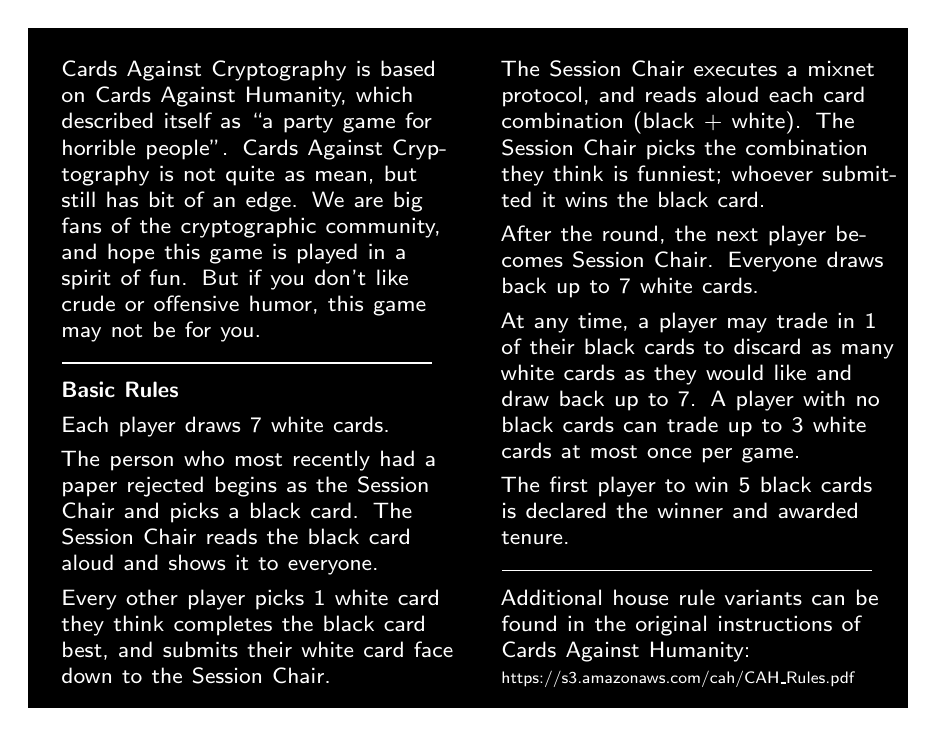
\begin{tikzpicture}[yscale=-1]

\renewcommand{\baselinestretch}{0.785}

\drawbackground

\newcommand{\myfont}{\sffamily\fontsize{8}{8}\selectfont }

% first page
\node [cardfg,below right,text width=1.96in] at (0.12in, 0.12in) {
	{\myfont
	Cards Against Cryptography is based on Cards Against Humanity, which described itself as ``a party game for horrible people''.  Cards Against Cryptography is not quite as mean, but still has bit of an edge.  We are big fans of the cryptographic community, and hope this game is played in a spirit of fun.  But if you don't like crude or offensive humor, this game may not be for you.}

	{\tikz \draw [line width=0.5pt,color=cardfg] (0,0)--+(1.85in,0);}

	\smallskip

	{\myfont
	\textbf{Basic Rules}
	}

	\smallskip

	{\myfont
	Each player draws 7 white cards.
	}

	\smallskip

	{\myfont
	The person who most recently had a paper rejected begins as the Session Chair and picks a black card.  The Session Chair reads the black card aloud and shows it to everyone.
	}

	\smallskip

	{\myfont
	Every other player picks 1 white card they think completes the black card best, and submits their white card face down to the Session Chair.
	}

};
% second page
\node [cardfg,below right,text width=1.96in] at (2.2in + 0.12in, 0.12in) {
	{\myfont
	The Session Chair executes a mixnet protocol, and reads aloud each card combination (black + white).  The Session Chair picks the combination they think is funniest; whoever submitted it wins the black card.
	}

	\smallskip

	{\myfont
	After the round, the next player becomes Session Chair.  Everyone draws back up to 7 white cards.
	}

	\smallskip

	{\myfont
	At any time, a player may trade in 1 of their black cards to discard as many white cards as they would like and draw back up to 7.  A player with no black cards can trade up to 3 white cards at most once per game.
	}

	\smallskip

	{\myfont
	The first player to win 5 black cards is declared the winner and awarded tenure.
	}

	{\tikz \draw [line width=0.5pt,color=cardfg] (0,0)--+(1.85in,0);}

	\smallskip

	{\myfont
	Additional house rule variants can be found in the original instructions of Cards Against Humanity:
	}

	{\sffamily\fontsize{6.5}{6}\selectfont
	https://s3.amazonaws.com/cah/CAH\_Rules.pdf
	}


};
\end{tikzpicture}
\end{document}
